% Assignment 4 - Dual-core vector add and timing
% UniCa - Advanced Embedded Systems (AES)

\documentclass[11pt,a4paper]{article}
\usepackage[utf8]{inputenc}
\usepackage[T1]{fontenc}
\usepackage[english]{babel}
\usepackage{geometry}
\usepackage{graphicx}
\usepackage{float}
\usepackage{booktabs}
\usepackage{listings}
\usepackage{hyperref}
\usepackage{xcolor}
\usepackage{fancyvrb}

\geometry{margin=2.5cm}
\graphicspath{{figures/}}

\title{Assignment 4 \\ Dual-core vector addition and timing}
\author{Matteo Tuzi \\ Student ID: 70/90/00490 \\ \medskip Course: Advanced Embedded System}
\date{\today}

\begin{document}
\maketitle
\tableofcontents
\newpage

%=============================================================================
\section{Purpose of the assignment}
%=============================================================================

The assignment requires implementing a bare-metal application on Zynq in which the two ARM Cortex-A9 cores cooperate to compute a vector sum $C = A + B$. Two execution modes are compared:
\begin{itemize}
  \item \textbf{Sequential:} a single core (Core~0) computes the entire vector $C$.
  \item \textbf{Parallel:} Core~0 computes the first half of $C$, Core~1 the second half; synchronisation is achieved via flags in shared memory.
\end{itemize}
The goal is to measure execution time with the ARM Global Timer and derive the speedup.

\newpage
%-----------------------------------------------------------------------------
\subsection{DDR memory map}
%-----------------------------------------------------------------------------
The following figures show the DDR region layout for the master (Core~0) and the worker (Core~1), as configured in the linker scripts.

\begin{figure}[htbp]
  \centering
  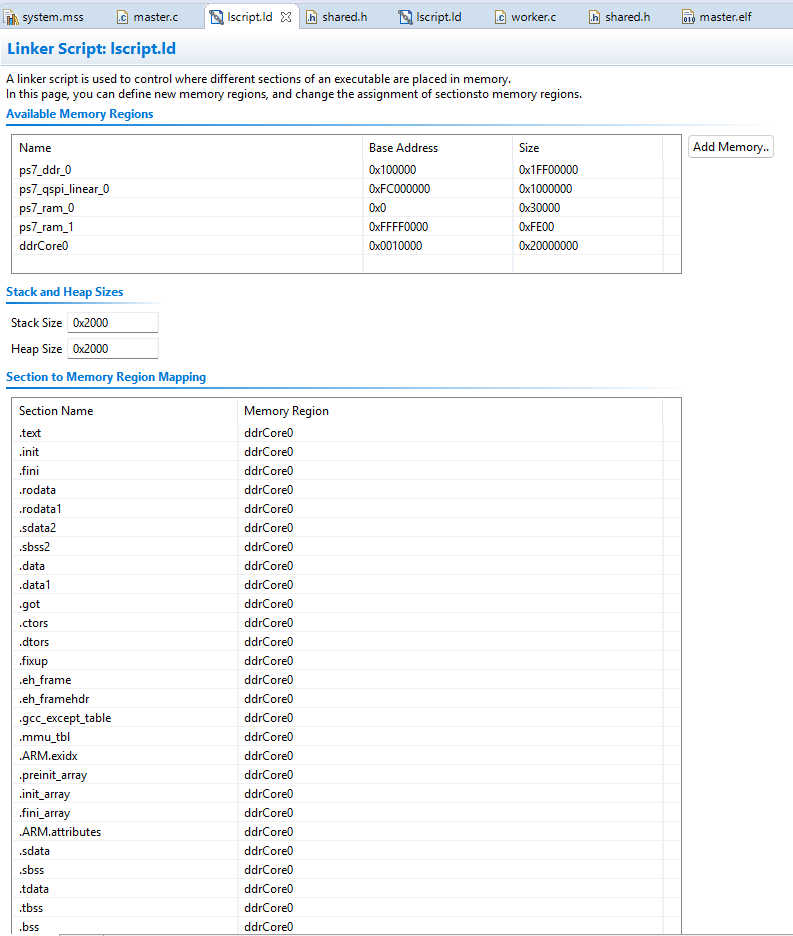
\includegraphics[width=0.85\textwidth]{ddrCore0}
  \caption{DDR memory Core0 (master).}
  \label{fig:ddr_core0}
\end{figure}

\begin{figure}[htbp]
  \centering
  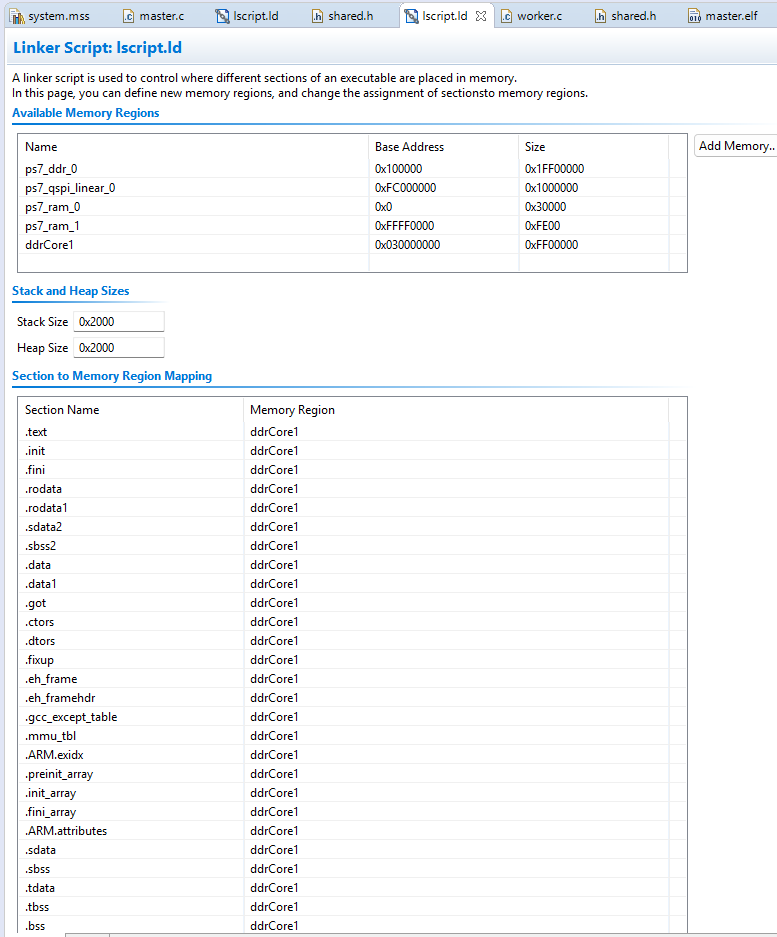
\includegraphics[width=0.85\textwidth]{ddrCore1}
  \caption{DDR memory Core1 (worker).}
  \label{fig:ddr_core1}
\end{figure}

\newpage
%=============================================================================
\section{Platform and tools}
%=============================================================================

\begin{itemize}
  \item \textbf{Board:} Zybo Z7 (Zynq-7000, dual ARM Cortex-A9).
  \item \textbf{Environment:} Xilinx SDK or Vitis; serial terminal 115200 8N1.
  \item \textbf{Peripherals:} Shared DDR, ARM Global Timer, AXI GPIO (button), UART.
\end{itemize}

The two cores use separate linker scripts: the master uses one DDR region (e.g.\ ddrCore0), the worker another (e.g.\ ddrCore1). The shared memory region (e.g.\ from \texttt{0x2F100000}) must not be assigned to any section by the linkers.

%-----------------------------------------------------------------------------
\subsection{Build configuration (optimisation -O3)}
%-----------------------------------------------------------------------------
The \textbf{master} and \textbf{worker} applications were built with \textbf{optimisation -O3} (Optimize most). In Xilinx SDK/Vitis: \texttt{Project $\rightarrow$ Properties $\rightarrow$ C/C++ Build $\rightarrow$ Settings $\rightarrow$ Optimization}, set level \texttt{-O3} for both projects.

With -O3 the compiler enables aggressive optimisations and vectorisation (\texttt{-ftree-vectorize}, \texttt{-mvectorize-with-neon-quad}) applies to the serial loop; the worker also runs its half of the vector efficiently, reducing the time the master waits in \texttt{done1}. A Debug (-O0) build would yield much higher parallel cycles and an artificially low speedup.

\begin{figure}[htbp]
  \centering
  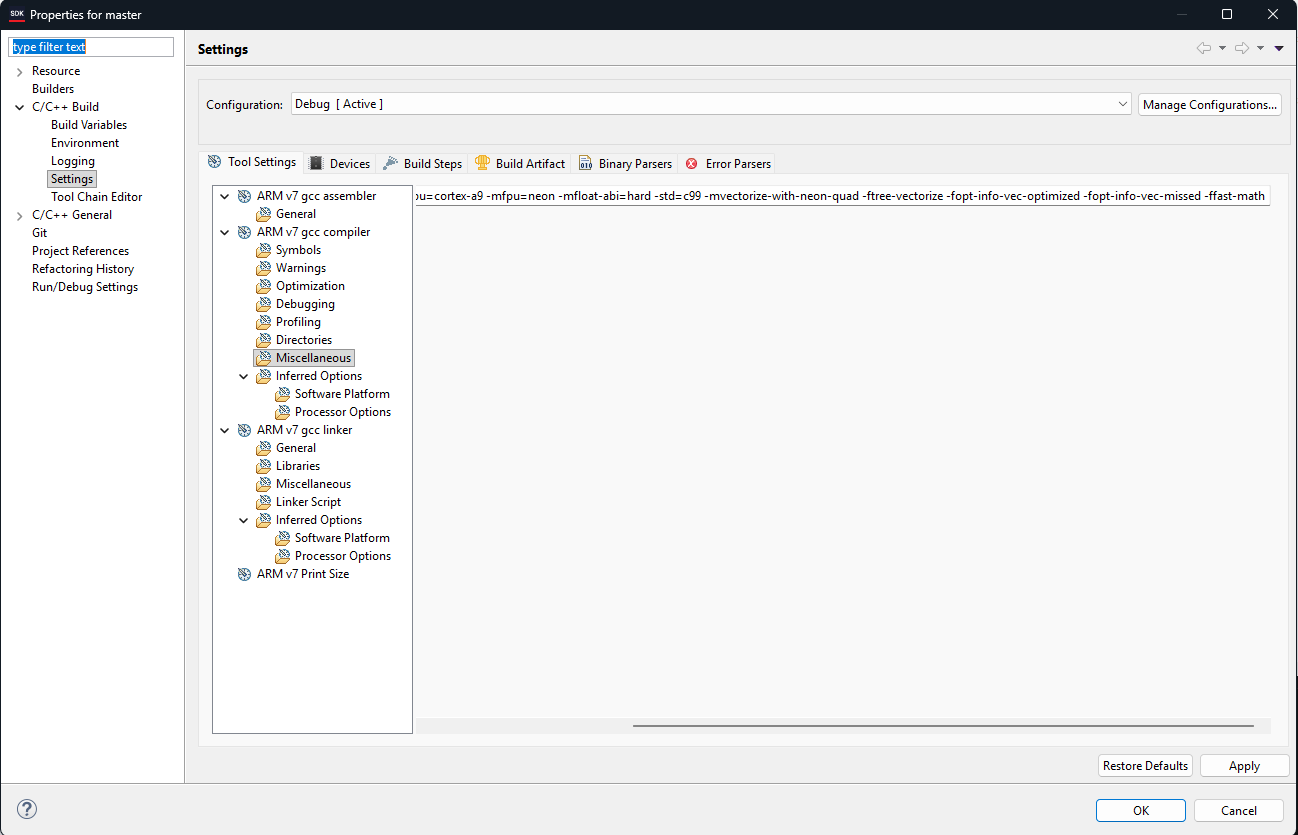
\includegraphics[width=0.9\textwidth]{master_compiler}
  \caption{Compiler options for master project (-O3 and NEON flags).}
  \label{fig:master_compiler}
\end{figure}

\begin{figure}[htbp]
  \centering
  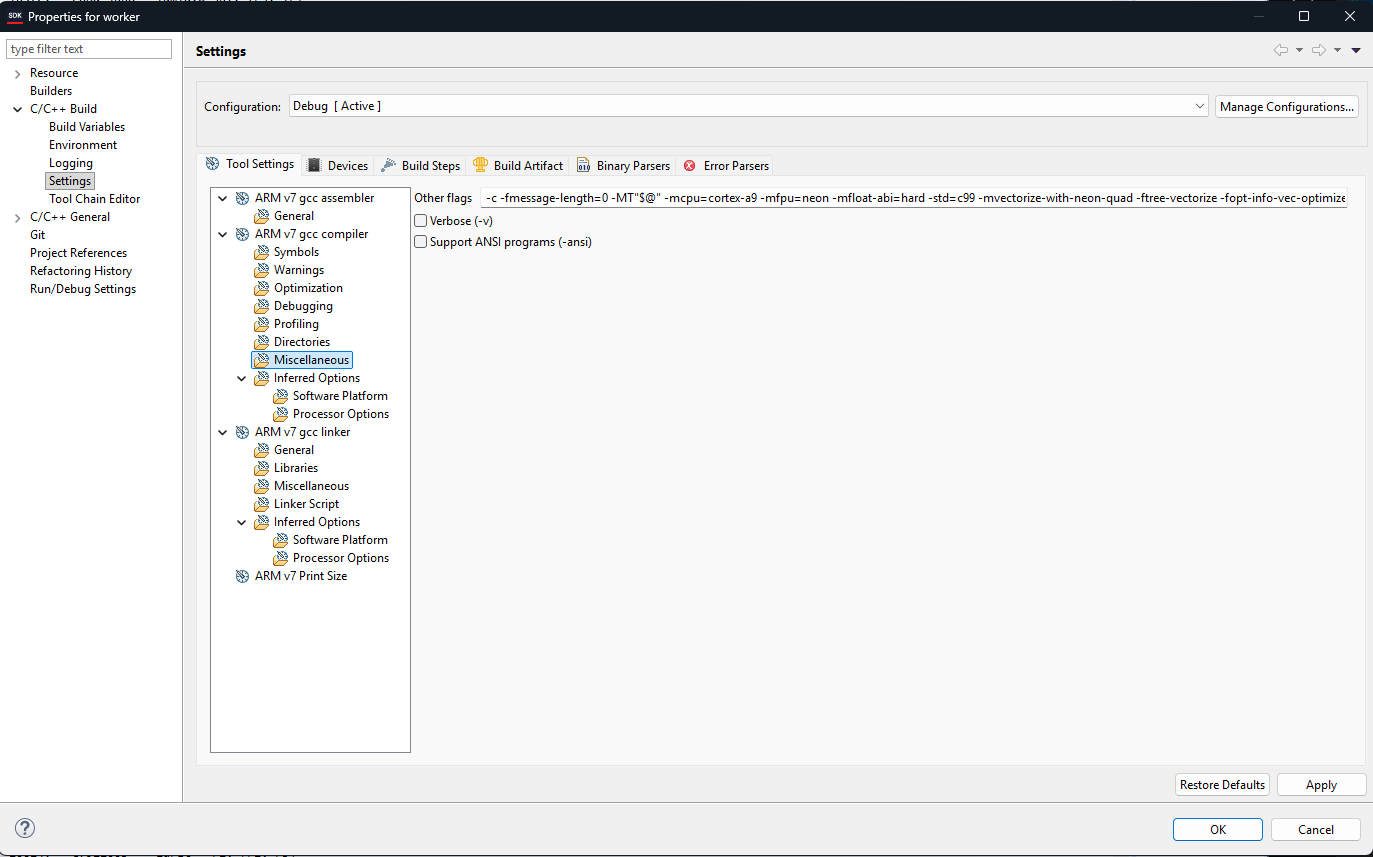
\includegraphics[width=0.9\textwidth]{worker_compiler}
  \caption{Compiler options for worker project (-O3 and NEON flags).}
  \label{fig:worker_compiler}
\end{figure}

%-----------------------------------------------------------------------------
\subsection{Run configuration / System Debugger}
%-----------------------------------------------------------------------------
The debug session uses a \textbf{System Debugger} configuration: \texttt{master.elf} is loaded on Core~0 (ps7\_cortexa9\_0) and \texttt{worker.elf} on Core~1 (ps7\_cortexa9\_1), with FPGA programming and system reset enabled, so that both cores start correctly.

\newpage
%=============================================================================
\section{Software architecture}
%=============================================================================

\subsection{Master role (Core~0)}
The master disables caches, waits for the GPIO button, initialises vectors $A$, $B$ and flags in shared memory. It runs the vector add in serial mode and measures its cycles (baseline). Then it clears $C$, waits for \texttt{ready1}, sets \texttt{start}, computes the first half of $C$, waits for \texttt{done1}, measures the parallel-phase cycles, computes the speedup and checks that $C$ matches the serial result.

\subsection{Worker role (Core~1)}
The worker disables caches, initialises \texttt{ready1} and \texttt{done1}, immediately signals \texttt{ready1 = 1}, waits for \texttt{start}, computes the second half of $C$, sets \texttt{done1 = 1} and enters idle.

%-----------------------------------------------------------------------------
\subsection{Shared memory}
%-----------------------------------------------------------------------------
The structure in \texttt{shared.h} contains vectors \texttt{A}, \texttt{B}, \texttt{C} and flags \texttt{ready1}, \texttt{start}, \texttt{done0}, \texttt{done1}. The base address is defined by \texttt{SHARED\_BASE} (e.g.\ \texttt{0x2F100000U}).

\begin{figure}[htbp]
  \centering
  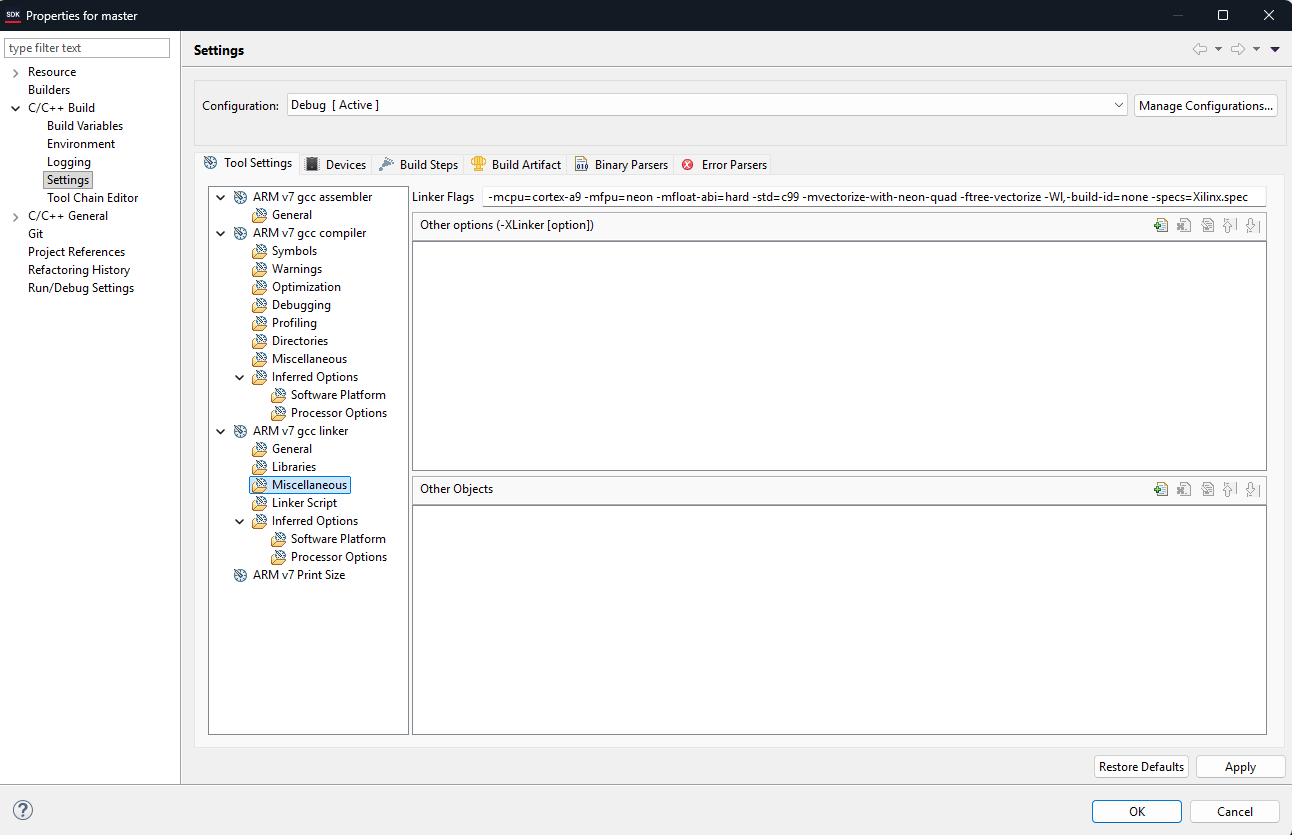
\includegraphics[width=0.85\textwidth]{master_linker}
  \caption{Master linker script: section placement in DDR Core0.}
  \label{fig:linker_master}
\end{figure}

\begin{figure}[htbp]
  \centering
  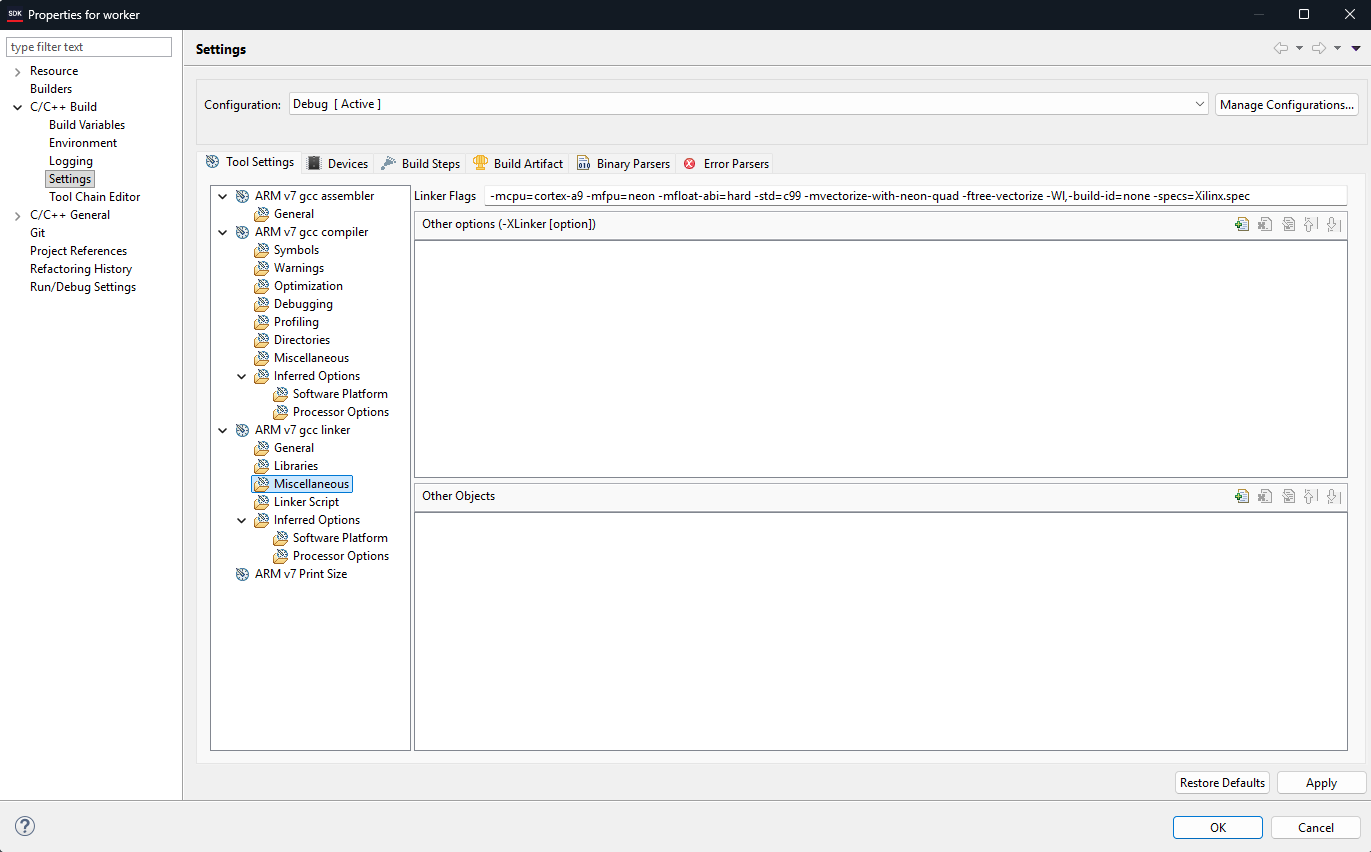
\includegraphics[width=0.85\textwidth]{worker_linker}
  \caption{Worker linker script: section placement in DDR Core1.}
  \label{fig:linker_worker}
\end{figure}

\newpage
%=============================================================================
\section{Timing measurement}
%=============================================================================

The Global Timer (32-bit register, \texttt{XPAR\_GLOBAL\_TMR\_BASEADDR + 0x00}) is used. For each phase the timer is read immediately before and after the block under measurement; the difference is the cycle count. Caches are disabled for deterministic timing. Results are expressed in cycles; the timer frequency is approximately 333\,MHz (platform-dependent).

%-----------------------------------------------------------------------------
\subsection{UART output}
%-----------------------------------------------------------------------------
The master output on the serial terminal (115200\,8N1) includes: boot message with \texttt{N}, serial and parallel run cycles, speedup and number of validation errors (zero if the parallel result matches the serial one). Figure~\ref{fig:uart_10} shows the example for \texttt{ARRAY\_SIZE=10}.

\begin{figure}[htbp]
  \centering
  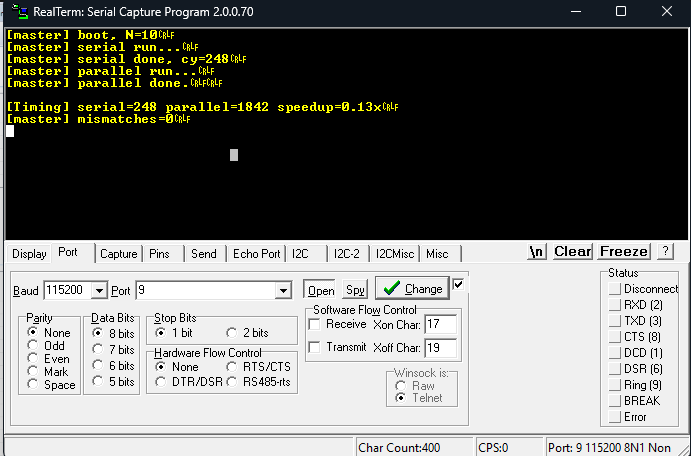
\includegraphics[width=0.9\textwidth]{test_array_10}
  \caption{UART output for ARRAY\_SIZE=10.}
  \label{fig:uart_10}
\end{figure}

%-----------------------------------------------------------------------------
\subsection{Results for different sizes}
%-----------------------------------------------------------------------------
Tests were run with \texttt{ARRAY\_SIZE} = 10, 100, 1000 and 5000. Below are the UART output screenshots for each size (sequential placement).

\begin{figure}[H]
  \centering
  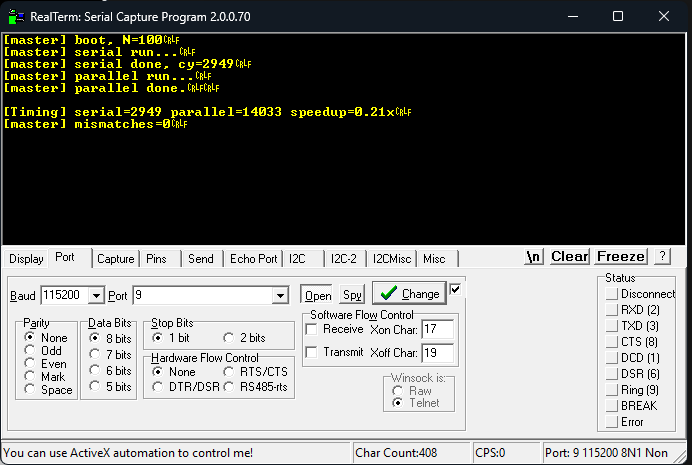
\includegraphics[width=0.9\textwidth]{test_array_100}
  \caption{UART output for ARRAY\_SIZE=100.}
  \label{fig:uart_100}
\end{figure}

\begin{figure}[H]
  \centering
  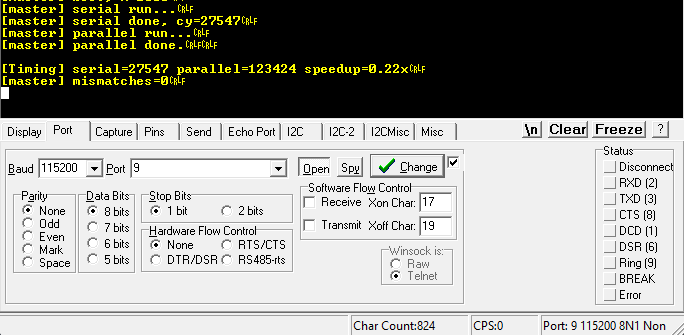
\includegraphics[width=0.9\textwidth]{test_array_1000}
  \caption{UART output for ARRAY\_SIZE=1000.}
  \label{fig:uart_1000}
\end{figure}

\begin{figure}[H]
  \centering
  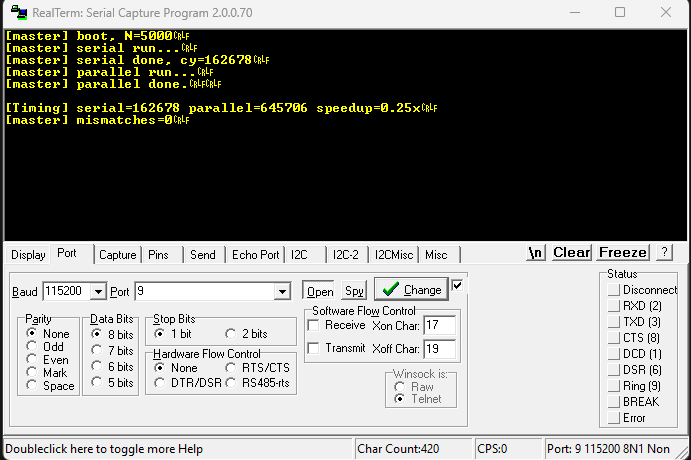
\includegraphics[width=0.9\textwidth]{test_array_5000}
  \caption{UART output for ARRAY\_SIZE=5000.}
  \label{fig:uart_5000}
\end{figure}

\paragraph{Summary table.} Values read from the screenshots for the four sizes tested.
\begin{center}
\begin{tabular}{cccc}
  \toprule
  ARRAY\_SIZE & Serial cycles & Parallel cycles & Speedup \\
  \midrule
  10   & 248    & 1\,842   & 0.13 \\
  100  & 2\,949 & 14\,033  & 0.21 \\
  1000 & 27\,547 & 123\,424 & 0.22 \\
  5000 & 162\,678 & 645\,706 & 0.25 \\
  \bottomrule
\end{tabular}
\end{center}

\newpage
%=============================================================================
\section{Interpretation of results}
%=============================================================================

Results for \texttt{ARRAY\_SIZE} = 10, 100, 1000 and 5000 show that parallel execution (two cores) does not achieve a speedup close to 2x over the serial baseline. In many cases the parallel-phase cycles are comparable to or higher than the serial ones, so the speedup is $\leq 1$.

This behaviour is expected on an architecture with \textbf{shared DDR memory} and \textbf{disabled caches}: the vector add kernel is \textbf{memory-bound}, i.e.\ execution time is dominated by memory accesses rather than computation. Both cores access the same DDR, causing \textbf{bandwidth contention}; the benefit of having two cores working in parallel is therefore limited by available bandwidth. With small \texttt{ARRAY\_SIZE} (10, 100) the \textbf{synchronisation overhead} (waiting for \texttt{ready1}, \texttt{start}, \texttt{done1}) can be comparable to compute time, further worsening the serial/parallel ratio. As vector size increases, useful work grows but contention on shared memory remains the limiting factor.

\newpage
%-----------------------------------------------------------------------------
\subsection{Assembly verification and NEON auto-vectorisation}
%-----------------------------------------------------------------------------
The serial code (\texttt{vec\_add\_serial}) was compiled with -O3 optimisation and NEON vectorisation flags. Inspection of the \texttt{master.elf} disassembly confirms the presence of \textbf{ARM NEON instructions} in the loop: \texttt{vld1.32} (vector load), \texttt{vadd.i32} (32-bit integer vector add), \texttt{vst1.32} (vector store). The compiler therefore applied auto-vectorisation to the serial loop, exploiting data-level parallelism (SIMD); this reduces the number of instructions executed per element but does not remove the shared-memory bottleneck in the parallel phase.

\begin{figure}[htbp]
  \centering
  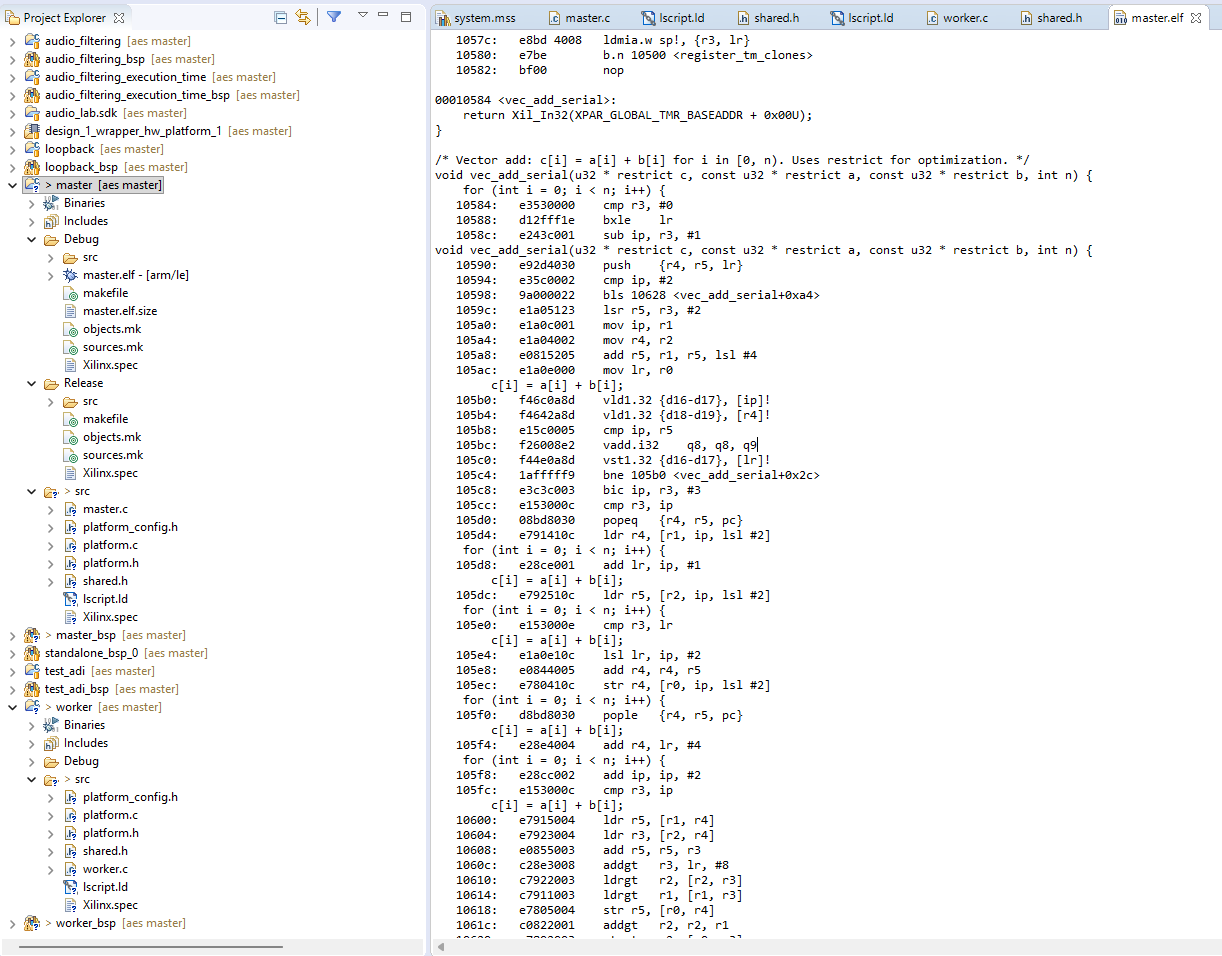
\includegraphics[width=0.9\textwidth]{disassembler}
  \caption{Disassembly of the serial function with NEON instructions (vld1.32, vadd.i32, vst1.32).}
  \label{fig:disasm}
\end{figure}

\newpage
%=============================================================================
\section{Conclusions}
%=============================================================================

The assignment led to implementing a bare-metal dual-core application on Zynq with coordination via shared memory and software flags. Serial and parallel execution of the vector add were compared, measuring cycles with the ARM Global Timer and verifying that the parallel result matches the serial one (zero errors).

The results confirm that, without caches and with shared DDR, a memory-bound kernel such as vector add does not benefit significantly from two-core parallelism: speedup remains limited or below 1 due to bandwidth contention. Building with -O3 and using NEON improves serial performance, but the main limit remains the memory architecture. The experiment is therefore consistent with the expected behaviour and with the literature on memory-bound workloads on embedded multi-core systems.

\end{document}
